% -*- fill-column: 85; -*-
%!TEX root = ../dissertation.tex

\section{Evaluation}
\label{s:eval}

\begin{figure*}
  \centering
	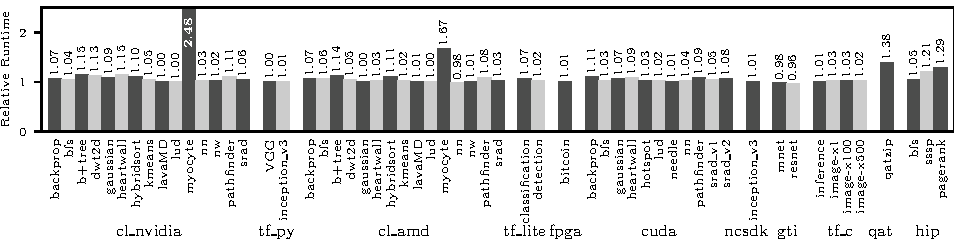
\includegraphics[width=\textwidth]{ava/data/end2end/end2end_all.pdf}
    \vspace{-1.75em}
	\caption{End-to-end execution time on virtualized APIs or accelerators normalized to native execution time. \lstinline|tf_py| is the handwritten TensorFlow Python API remoting with \AvA API-agnostic components.}
	\label{fig:end2end}
	%\vspace*{-0.75em}
\end{figure*}

\begin{figure}
	\centering
	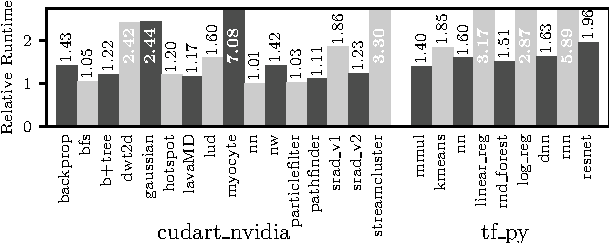
\includegraphics[width=\columnwidth]{ava/data/end2end/end2end_cudart.pdf}%
	\vspace*{-.1em}
	\caption{End-to-end execution time on virtualized CUDART and CUDA-accelerated TensorFlow APIs normalized to native execution time.}
	\label{fig:end2end_cudart}
	%\vspace*{-.6em}
\end{figure}

\begin{comment}
\amp{Move these the section that addresses them if we want to use them explicitly.}
Our evaluation focuses on:
\begin{compactitem}
\item Quantifying the development effort involved in virtualizing an accelerator API using \AvA.
\item Understanding \AvA's efficacy for different API frameworks.
\item Application performance on a \AvA-virtualized accelerator.
\item The sources of overhead in a virtual stack constructed with \AvA, and possible optimizations.
\item \AvA's ability to enforce resource policies (e.g., fair sharing).
\item The performance of \AvA's record-and-replay scheme.
\end{compactitem}
\end{comment}


\AvA was evaluated on an Intel Xeon E5-2643 CPU with 128~GiB DDR4 RAM, using
Ubuntu~18.04 LTS, and Linux 4.14 with modified KVM and vhost modules.
Guest VMs were assigned 4 virtual cores, 4~GiB memory, 30~GB disk space, and ran Ubuntu~18.04 LTS with the stock Linux 4.15 kernel.
\workers and VMs were co-located on the same server for all experiments except live migration and the FPGA benchmarks.
Experiments involving a Google Cloud TPU were carried out on a Google Compute Engine instance with 8 vCPUs (SkyLake), 10~GiB memory, and a disaggregated Cloud TPU v2-8 in the same data center.
The guest VM was located on the same instance via nested virtualization.
Experiments for the custom FPGA API were done on an AWS F1 \lstinline|f1.2xlarge| instance (with 1 Virtex UltraScale+ FPGA, 8 vCPUs, and 122 GiB memory).
For live migration, a second similar server was used as the remote machine, and the servers were directly connected by 10 Gigabit Ethernet.

\subsection{Development Effort}
\label{s:eval_effort}

%Traditional API forwarding schemes have had trouble keeping up with the rate
%of evolution of framework APIs due to the massive engineering effort needed.
%\AvA is designed to assist virtualization engineers by automatically
%generating the guestlib and \worker for each API from a specification written
%in \Lapis.

\definecolor{Gray}{gray}{0.9}
\begin{table}
	\footnotesize
    \newcolumntype{\N}{S[table-format=4.0, table-alignment = right, table-auto-round = true]}
    \newcolumntype{\n}{S[table-format=1.0, table-alignment = right, table-auto-round = true]}
    \setlength{\tabcolsep}{3pt}
	% \begin{tabular}{>{\raggedright\arraybackslash}m{7.4em}m{0.8em}\n\N\N >{\raggedright\arraybackslash}m{4.0em}>{\raggedright\arraybackslash}m{7.4em}}
	\begin{tabular}{ccccccc}
    \toprule
	API                         & Gen              & {\#}                 & {LoC}                  & {Churn}                 & Benchmark                & Hardware                                      \\
	\midrule
	\multirow{2}{*}{OpenCL~1.2} & \cross \cellcolor{Gray} & {\cellcolor{Gray}}39 & {\cellcolor{Gray}}7514 & {\cellcolor{Gray}}14318 & \multirow{2}{*}{Rodinia} & \multirow{2}{7em}{NVIDIA~GTX~1080 AMD~RX~580} \\
                                & \checkmark       & 38                   & 1060                   & 2868                    &                          &                                               \\
	CUDA 10 Driver              & \checkmark       & 16                   & 266                    & 410                     & Rodinia                  & NVIDIA~GTX~1080                               \\
	CUDA 10 Runtime             & \checkmark       & 93                   & 1358                   & 1973                    & Rodinia                  & NVIDIA~GTX~1080 								\\
	TensorFlow~1.12~C           & \checkmark       & 46                   & 501                    & 887                     & Inception                & NVIDIA~GTX~1080                               \\
	TensorFlow~1.13~Py          & \cross           & {\scriptsize n/a}    & 3245                   & 5972                    & VGG-net Inception        & Google~Cloud TPU v2-8                         \\
	TensorFlow~1.14~Py          & \checkmark       & 111                  & 1865                   & 2557                    & Neural networks          & NVIDIA~GTX~1080 								\\
	TensorFlow Lite~1.13        & \cross           & {\scriptsize n/a}    & 1295                   & 2005                    & Official examples        & Coral Edge~TPU                                \\
	NCSDK~v2                    & \checkmark       & 26                   & 479                    & 1279                    & Inception                & Movidius~NCS v1                         \\
	GTI SDK~4.4                 & \checkmark       & 38                   & 284                    & 568                     & Official examples    & Gyrfalcon 2803 Plai Plug                         \\
	Custom FPGA on AmorphOS~\cite{amorphos}     & \checkmark       & 4                    & 30                     & 40                      & BitCoin  & AWS~F1                                        \\
	QuickAssist~1.7             & \checkmark       & 19                   & 444                    & 676                     & QATzip                   & Intel~QAT 8970                      \\
	HIP                         & \checkmark       & 41                   & 624                    & 990                     & Galois~\cite{tao}        & AMD~Vega~64                                   \\
	\bottomrule
	\end{tabular}
	\caption{Development effort for forwarding different APIs, along with the benchmarks~\cite{inceptionv3,vggnet,rodinia} and hardware used to evaluate them.
      The \textbf{\#} column indicates the number of API functions supported.
      The Python APIs are forwarded dynamically, making \# inapplicable.
      \textbf{Gen} indicates whether the API forwarding was generated by \CAvA or was written by hand.
      \textbf{LoC} is the number of lines of code (including blank lines and comments) in the \CAvA specification or C/Python code.
      \textbf{Churn} is the total number of lines modified in commits.
      % Inception is Inception~v3~\cite{inceptionv3}.
      % VGG-net is from \cite{vggnet}.
      % Rodinia is from \cite{rodinia}.
    }
	\label{tab:apis-and-accelerators}
	\vspace*{-.2em}
\end{table}

\begin{comment}
\begin{table}
	\footnotesize
	\begin{tabularx}{\columnwidth}{p{8em}p{4em}P{4em}p{4em}p{4em}}
	\toprule
	API Name & \#Supported   & Generated & L.o.C. & Churn\\
	\midrule
	OpenCL~1.2               & 39    &            & 7,514 & 14,318\\
	\rowcolor{Gray}
	OpenCL~1.2               & 38    & \checkmark & 1,060 & 2,868\\
	CUDA 10.0 Driver         & 16    & \checkmark & 266   & 410\\
	\rowcolor{Gray}
	Tensorflow~1.12 (C)      & 46    & \checkmark & 501   & 887\\
	Tensorflow~1.13 (Py)     & {n/a} &            & 3,245 & 5,972\\
	\rowcolor{Gray}
	Tensorflow Lite~1.13     & {n/a} &            & 1,295 & 2,005\\
	NCSDK~v2                 & 26    & \checkmark & 479   & 1,279\\
	\rowcolor{Gray}
	Custom FPGA API          & 4     & \checkmark & 30    & 40\\
	QuickAssist~1.7          & 19    & \checkmark & 444   & 676\\
	\rowcolor{Gray}
	HIP                      & 41    & \checkmark & 624  0 & 990\\
	\bottomrule
	\end{tabularx}
	\caption{Development effort for forwarding different APIs. Number of APIs supported is not applicable to Python APIs as they are forwarded dynamically. The \textbf{Generated} column indicates whether the API forwarding was generated by \CAvA or was written by hand. \textbf{L.o.C.} is the number of lines of code in the \CAvA specification or C/Python code. \textbf{Churn} is the total number of lines modified in commits.}
	\label{tab:api-dev-effort}
\end{table}
\end{comment}


We present our experience building API remoting systems by hand and with
\CAvA as evidence of the significant reduction in developer effort
\CAvA provides.
We characterize developer effort to virtualize \numframeworks APIs and \numaccelerators devices in terms of the lines of code in the \CAvA specifications or C/Python code (\texttt{LoC} in Table~\ref{tab:apis-and-accelerators}), and the number of lines of code modified (\textbf{Churn} in Table~\ref{tab:apis-and-accelerators}) during development (counted from commits).
Building an API remoting system for OpenCL, which supports all the APIs needed to run the Rodinia~\cite{rodinia} benchmarks, by hand took more than 3 developer-months, and spanned 7,514 LoC (see row 1 of Table~\ref{tab:apis-and-accelerators}).
Supporting the same subset of OpenCL with \AvA, took a single developer a little over a week, and the resulting API specification was 1,060 LoC long.
%The reduction in both time spent and lines of code written and modified to virtualize the OpenCL API %demonstrates that \CAvA reduces the effort required to virtualize a compute accelerator API.
Even in cases where we couldn't leverage \AvA---%
TensorFlow and TensorFlow Lite Python APIs---%
leveraging \AvA's API-agnostic components enabled us to build a \hira system with reasonable effort (3,245 lines of Python code and 2 developer weeks for TensorFlow Python).

\subsection{End-to-end Performance}

% We measured the APIs and accelerators that we virtualized with \AvA using the benchmarks described in Table~\ref{tab:apis-and-accelerators}.
Figure~\ref{fig:end2end}--\ref{fig:end2end_cudart} shows the end-to-end runtime, normalized to native, for all benchmarks, accelerator and API combinations we support (see Table~\ref{tab:apis-and-accelerators}).
\AvA introduces modest overhead for most workloads.
%geometric mean overhead is 8.6\%.
Excluding \texttt{myocyte}, the Rodinia OpenCL benchmarks on NVIDIA GTX 1080
GPU slowed down by 7\% on average.
The outlier, \texttt{myocyte} has over 2$\times$ overhead because it is extremely \textbf{call-intensive}---it makes over 200,000 calls in \SI{18.5}{\second}; most others make between 30 and 3,000 calls.
For comparison, FlexDirect sees 3.3$\times$ slowdown for \texttt{myocyte};
GPUvm sees 100$\times$ or more for call-intensive workloads~\cite{yu2017fullvirt}.
\texttt{Myocyte} experienced lower overhead on the AMD Radeon RX
580 GPU, as the kernels executed 3$\times$ slower, allowing more of
\AvA's overheads to be amortized.
The benchmarks for CUDA runtime API and CUDA-accelerated TensorFlow are mostly call-intensive.
The geometric mean overhead is 79.6\%, 4$\times$ faster than FlexDirect.

The TensorFlow benchmarks for the handwritten Python API remoting system, and Movidius benchmarks show low overhead---%
0\% overhead on VGG-net running on TensorFlow Python (Cloud TPU), and 7\% slowdown for image classification on TensorFlow Lite (Coral Edge TPU)---%
as they are \textbf{compute-intensive}. Each offloaded kernel performs a lot of computation per byte of data transferred, with relatively few API calls.
The Gyrfalcon benchmarks enjoy a slight speedup as time spent loading and initializing the library are eliminated by using a pre-spawned \worker pool.
The QuickAssist accelerator proved challenging to virtualize, as it is a high-data-rate kernel-bypass encryption/compression accelerator.
Applications that run on this device are \textbf{data-intensive}: computation per transferred byte is very low.
We ran the Intel QATzip compression application on the Silesia corpus~\cite{silesia} using synchronous QAT APIs: while the application only experienced a 1.38$\times$ end-to-end runtime slowdown, its throughput was 2.2$\times$ lower on average.
\AvA was not able to keep up with the high throughput of the device, due to data transfer and marshalling overheads, as the time spent transferring data between the guest and the host was equivalent to compute time on the accelerator.
We are exploring zero-copy techniques to ameliorate this. We note that QAT on \AvA is fair, unlike the onboard SR-IOV support.

% QATzip with different datasets on QuickAssist API,
% for which the average end-to-end overhead is 38.8\%,
% but the throughput for data compression has 2.2$\times$ slowdown.
% \hyu{@Amogh, explain..}


% \subsubsection{Workload Characteristics}\hyu{Address when we gather up}
\label{s:micro_benchmark}

\begin{figure}
  \centering
	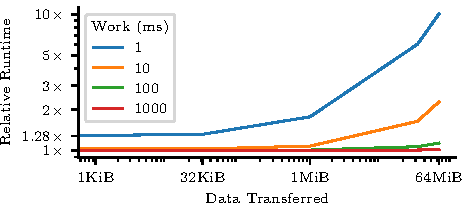
\includegraphics[width=\columnwidth]{ava/data/microbenchmark/overhead_plot.pdf}%
    \vspace*{-.5em}
	\caption{Overhead on a micro-benchmark with varying work per call and data per call. The plot is log-log and the trend is linear.
    % \aak{what is the data normalized to? How much data was computed on, i.e., does this represent call-intensive at 1KiB and data-intensive at 64MiB?}
    }
	\label{fig:microbenchmark_overhead}
	%\vspace*{-0.5em}
\end{figure}

\subsection{Micro-benchmarks}

To understand performance trade-offs for \AvA,
%suitability for compute-intensive, data-intensive, and call-intensive applications,
we ran a micro-benchmark that transferred different amounts of data per call and simulated accelerator computation for different lengths of time by spinning on the host.
Figure~\ref{fig:microbenchmark_overhead} shows compute-intensive applications (represented by the lines for 100~ms and 1,000~ms of work) suffer the lowest overhead, as data transfer is amortized by time computing on that data.
Data-intensive applications (represented by the 1~ms and 10~ms lines) experience severe slowdowns as the data transferred per call increases, such as when 64~MiB is moved for only 1~ms of compute.
Call-intensive applications transfer little data and have short kernels, so control transfer dominates execution, (e.g. 28\% overhead on 1~ms calls with no data).


\begin{comment}
\aak{commented this out cos we've expressed the same thing more compactly above.}
\paragraphbe{Compute-intensive} applications have long device computations with relatively little data transferred per call and infrequent calls.
	This kind of applications are offloading compute kernels to an accelerator with an API (e.g., OpenCL and CUDA).
    Specialized machine learning frameworks~\cite{caffe,graphcore,pytorch_use_gpu,tensorflow_use_gpu,abadi2016tensorflow,cyphers2018intel} are also compute-intensive.
    %, like Tensorflow, Caffe2, PyTorch, Poplar, Nervana, and nGraph,
	In compute-intensive APIs, the overheads of data transfer and API forwarding are amortized by the long execution time, leading to low overall overhead.\hyu{Shrink}

\paragraphbe{Data-intensive} applications have large data transfers and relatively short compute kernels,
	so the data transfer overhead cannot be amortized.
	Some OpenCL and CUDA workloads fall into this category,
	as the device compute time is much shorter than the data transfer time;
    kernel bypass APIs (e.g., Intel QAT) often fall into this category as well.
	This overhead could be reduced with zero-copy data transfer.

\paragraphbe{Call-intensive} applications have short frequent API calls.
    A common example of this is the network communication with a NIC API.
    This type of API is not suitable for API remoting, because the per call transport overhead is unacceptable.
\end{comment}

\begin{figure}[!th]
	\centering
	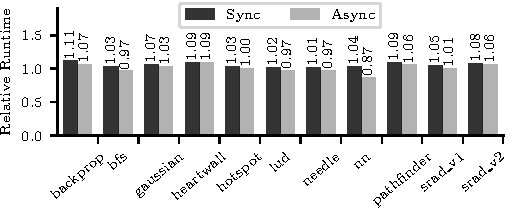
\includegraphics[width=\columnwidth]{ava/data/end2end/end2end_async.pdf}%
	\vspace*{-.5em}
	\caption{End-to-end runtime of CUDA benchmarks (relative to native) using synchronous and asynchronous specifications.}
	\label{fig:eval_async}
	\vspace*{-1em}
\end{figure}

\subsubsection{Asynchrony Optimizations}
\label{s:opt_eval}

% We measured the system using OpenCL benchmarks on NVIDIA GTX 1080 GPU with two transport channels, shared memory and VM socket, with or without asynchrony calls.
% In most cases, shared memory has obvious improvement to the performance, 20\% speedup in average,
% because VM socket with virtio-vsock device suffers from low throughput due to the limited size of receive buffers and the share of the single RX/TX virt-queue pair among all applications in the same VM.
% Benchmarks such as nw and pathfinder suffer from slowdown with shared memory,
% because they transfer small amount of data, and the cost of shared memory management cannot be counteracted by the reduction of data copies.
% \subsection{Asynchrony}
% \label{s:asynchrony}
% \AvA allows functions annotated as

% Some synchronous  may safely be executed asynchronously:
Synchronous APIs calls that have no output of any kind remain semantically correct if executed asynchronously.
For example, \lstinline|clSetKernelArg| is a synchronous OpenCL API,
but can be forwarded asynchronously to reduce the overhead of these calls. % at the cost of fidelity:
The application's execution will not be faithful to native execution, as the library would return immediately after the command is sent to the \worker.
Any resulting errors will be delivered from a later API call.
Similar techniques were applied in vCUDA (lazy RPC)~\cite{vCUDA} and rCUDA (API batching)~\cite{rCUDA}. % with the same loss of fidelity.

We annotated several synchronous APIs---\lstinline[breaklines=true,escapechar=|]@cuLaunchKer@\-\lstinline@nel@, \lstinline@cuMemcpyHtoD@, and resource free functions---as asynchronous.
% The errors in these calls may be reported in a later call,
% but successful execution produces correct results.
Figure~\ref{fig:eval_async} shows that this optimization results in a 5\% speedup on average (geometric mean) in end-to-end runtime (normalized to native) for CUDA Rodinia benchmarks.
%Several benchmarks (e.g., \textit{nn}) experience speedup because \aak{figure out why nn is so fast.} \hyu{Fix: Transfer, execution overlap; release non-blocking}.

\subsection{Scalability}
\begin{figure}
	\centering
	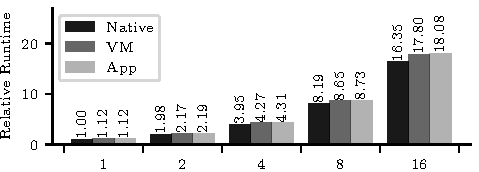
\includegraphics[width=.95\linewidth]{ava/data/scalability/scalability.pdf}%
	\vspace{-0.4em}
	\caption{Scalability of multiple VMs running a single application each, and multiple applications in a single VM,  with \AvA. Runtime is relative to running the same number of applications natively.}
	\label{fig:scalability}
	\vspace*{-.25em}
\end{figure}

% \AvA provides scalability and concurrency for simultaneous guest VMs and applications.
To evaluate scalability, we ran multiple instances of the OpenCL \texttt{gaussian} benchmark
simultaneously in a varying number of VMs with a NVIDIA GTX 1080 GPU. The \texttt{gaussian} benchmark fully saturates the GPU.
The \AvA overhead ($\sim$10\%) does not increase as the number of VMs or applications increases,
as shown by the near-perfect scaling in Figure~\ref{fig:scalability}.
The GPU kernel execution has an average 5.7\% slowdown each time the number of VMs and applications is doubled.
% , while the end-to-end performance does not change.
This slowdown is small due
better utilization of the physical device and other system resources.
%, i.e.,
% an application in one VM can utilize the GPU when other applications are not.
% \reviewer{A}{What is the intuition behind the perfect scaling?}

Accelerators without process-level protection or sharing support (e.g., Intel Movidius NCS) do not scale will with \AvA, as multiple applications attempting to use the device have to be serialized.
\AvA added modest overheads (11\%) in a case where 4 VMs were all running inception on the NCS v1. We note that \AvA still provides benefit by enabling a hypervisor to expose and share the device across guest VMs.

% \begin{comment}
\subsection{API Rate Limiting}
\label{s:eval_rate_limit}

To measure the fairness achieved by \AvA, we repeatedly executed kernels drawn from six CUDA OpenCL benchmarks in pairs simultaneously in two VMs.
 % with virtualized NVIDIA GTX 1080 GPU.
The kernels last from 1~ms to 100~ms.
Figure~\ref{fig:fairness} shows the fairness of the execution with fixed-rate polling and feedback control method in 500-ms and 1-s measurement windows.
We compute the unfairness as
$\left|t_1-t_2\right| \mathbin{/} (t_1+t_2),$
where $t_i$ is the device time used by VM$_i$ in the time window.

% With the same size of time window, it is expected to see less fairness and smaller scheduling overhead with longer kernels as the GPU kernel is non-preemptible.
For fixed-rate polling ($p=5$~ms), median unfairness in a 1~s window is 2.6\%, and scheduling overhead was 7\%.
For feedback control ($a=1$~ms and $b=1/2$),
%The initial, minimum and maximum delays are set to 5~ms, 0.5~ms and 10~ms correspondingly.
median unfairness is 2.4\% in a \SI{1}{\second} measurement window, with 15\% overhead.

\begin{figure}
	\centering
    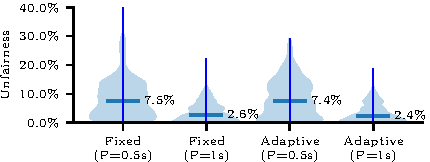
\includegraphics[width=\columnwidth]{ava/data/rate_limit/bias_plot.pdf}%
    \vspace{-.35em}
	\caption{Unfairness of the fixed and adaptive scheduling algorithms with two different measurement periods.
      The width of the shaded areas show the probability of the bias (unfairness) being a specific value in any given measurement window.
      The horizontal bar shows the median and the vertical line runs from the minimum to the maximum.}
	\label{fig:fairness}
\end{figure}


\subsection{Live Migration}

\begin{figure}
	\centering
	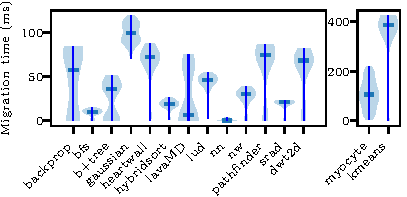
\includegraphics[width=\columnwidth]{ava/data/migration/time_plot.pdf}%
    % \vspace{-0.6em}
	% 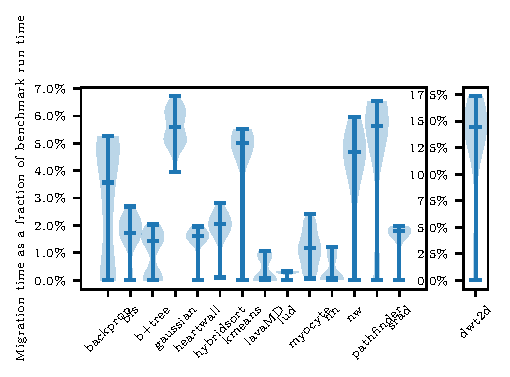
\includegraphics[width=\columnwidth]{ava/data/migration/factor_plot.pdf}
	\caption{Live migration downtime for single-threaded OpenCL benchmarks on NVIDIA GTX 1080.
      This downtime is in addition to the $\sim$\SI{75}{\milli\second} of downtime of the VM migration itself.
      Migration downtime does not include time spent waiting for executing kernels to complete (accounted as latency), as the application is still performing useful computation on the accelerator during that time.
      % The width of the shaded areas show the the probability of a migration taking that length of time.
      % The horizontal bar shows the median and the vertical line shows the range from minimum to maximum.
    }
	\label{fig:migration}
	%\vspace{-.5em}
\end{figure}

% To evaluate \AvA's
%live-migration scheme uses annotations and selective record-and-replay instead of replaying the entire application on the remote.
%To understand the efficacy of our method,
We live-migrated a VM with 4~GB memory, that was running OpenCL applications from the Rodinia benchmark suite, between two servers that were directly connected via a 10~Gib Ethernet link, both equipped with NVIDIA GTX 1080 GPUs.
Migration was triggered at random points in each benchmark, and the application could not make API calls for the duration of the migration.
Migrating the VM without \AvA or GPU usage takes \SI{19}{\second} with a \SI{75}{\milli\second} downtime on average.
% In the experiment, the migration is started at random points during the OpenCL application's lifetime,
% where the application is paused until the migration is done.
% Both servers had .

\begin{comment}
Migration was carried out in three pipelined stages:
the source \worker extracted explicit state from API objects, and then transferred recorded commands for implicit state and replacement commands for explicit state to the target \worker. The target \worker then replayed the transferred commands.
\aak{I think we don't need this here. We've already explained it in the migration section...}
\end{comment}

\begin{comment}
Migration samples for each benchmark:
backprop: 50
bfs: 50
b+tree: 50
dwt2d: 50
gaussian: 150
heartwall: 50
hybridsort: 50
kmeans: 50
lavaMD: 50
lud: 150
myocyte: 200
nn: 50
nw: 50
pathfinder: 50
srad: 50
\end{comment}

Figure~\ref{fig:migration} shows the downtime experienced by applications in the VM, not including downtime for migrating the VM itself.
200 samples were collected for \texttt{myocyte}, 150 for \texttt{gaussian} and \texttt{lud}, and 50 for all others.
% , based on the number of APIs calls made by the applications.

The dominant cost is command transfer and replay, but this cost is also affected by the size of the benchmark's state.
Figure~\ref{fig:migration} shows a bimodal distribution of downtime for most benchmarks. This is an artifact of applications allocating device memory before entering a steady execution state, and freeing it at termination.
% \amp{Don't the benchmarks also free the buffers during execution? If the buffers were ALL freed at the end I would expect a MUCH more spread out distribution.}
%\hyu{Most free buffers at the end. Gaussian and myocyte are exceptions.}
Migrations that occur before device memory allocation do not need to transfer significant state; migrations that occur after device memory allocation do.
% but migrations after buffer creation must copy all the resident buffers and their associated commands.

% Because our test servers are connected via a relatively slow TCP link, the transfer stage can be slow.
% For example, dwt2d allocates large device memory buffers, and the buffer transfer time exceeds the benchmark's length\amp{Is this still true with 10g?}.\hyu{Not true any more.}

%\aak{this paragraph is conflicting with the caption of the figure.}
%\hyu{One is downtime, one is latency.}
%\AvA needs to wait for in-flight calls to finish,
%introducing latency which can be as long as the kernel execution time in the worst case.
%The \textit{Kmeans} benchmark comprises a long-running GPU kernel, so its migration time is up to 425~ms.
%However, the pause time of the application does not include this latency, because during that time the application is still performing useful computation on the accelerator.
%For applications which must execute more than one kernel to fully utilize the device, this latency could increase the perceived downtime.
